\documentclass{beamer}
\usepackage[fontset=fandol]{ctex}
\usepackage{hyperref}
\usepackage[T1]{fontenc}
\usepackage{latexsym,amsmath,xcolor,multicol,booktabs,calligra}
\usepackage{graphicx,array}

\author{罗一逖、张子诺、朱云天、郑永祺}

\title{新兴科技革命下的技术追赶与技术差距研究}
\subtitle{以核能科学为例}
\institute{南京大学信息管理学院}
\date{2026年3月10日}
\usepackage{NJU}
\advisor{闵超}

\AtBeginSection[]{}
\AtBeginSubsection[]{}
\setbeamertemplate{navigation symbols}{}

\newcommand{\hi}[1]{\textcolor{njupurple}{\textbf{#1}}}
\newcommand{\capline}[1]{{\tiny #1}}

\begin{document}

\kaishu
\begin{frame}
    \titlepage
    \begin{figure}[htpb]
        \centering
        
\includegraphics[width=0.18\linewidth]{pic/NJU_Logo.png}
    \end{figure}
\end{frame}

\begin{frame}{汇报提纲}
    \tableofcontents
\end{frame}

\section{研究背景与意义}

\begin{frame}{研究背景与意义}
    \begin{columns}[T]
        \begin{column}{0.30\linewidth}
            \begin{block}{核心问题}
                \small
                在以核能科学为例的高精尖领域中，如何衡量各国之间的\hi{技术差距}，发掘技术追赶的\hi{路径和机制}？
            \end{block}
        \end{column}
        \begin{column}{0.30\linewidth}
            \begin{block}{研究方法}
                \small
                聚焦论文的\hi{自然语言文本}，结合\hi{文本分析}和\hi{网络分析方法}，构建多维度的\hi{技术追赶测度体系}，系统评估中国在核能科学领域的追赶进程。
            \end{block}
        \end{column}
        \begin{column}{0.30\linewidth}
            \begin{block}{核心目的}
                \small
                反映中国在核能为代表的新兴科技领域的追赶现状，揭示追赶的\hi{路径和机制}，为科技政策制定提供实证支持。
            \end{block}
        \end{column}
    \end{columns}
\end{frame}

\section{研究设计}

\begin{frame}{研究目标与证据链}
    \begin{columns}[T]
        \begin{column}{0.52\linewidth}
            \begin{itemize}
                \item 不是只比较\hi{发文量}，而是测度\hi{主题差距、结构差距、流动差距、前沿差距}。
                \item 核心问题：
                \begin{itemize}
                    \item 是否存在主题结构差距？
                    \item 追赶路径是否实现赶超？
                    \item 前沿能力是否存在差异？
                    \item 知识扩散机制是否不同？
                \end{itemize}
            \end{itemize}
            \begin{block}{样本口径}
                WoS 文献 \hi{25,794} 篇，1990--2026\\
                CN \hi{5,687}，US \hi{3,379}
            \end{block}
        \end{column}
        \begin{column}{0.43\linewidth}
            \begin{block}{证据链}
                文本嵌入\\
                \quad $\Downarrow$\\
                主题结构\\
                \quad $\Downarrow$\\
                追赶路径\\
                \quad $\Downarrow$\\
                前沿能力\\
                \quad $\Downarrow$\\
                知识传播
            \end{block}
        \end{column}
    \end{columns}
    \vspace{0.3em}
\end{frame}

\begin{frame}{目前阶段已经完成的工作}
    \begin{columns}[T]
        \begin{column}{0.48\linewidth}
            \begin{block}{1. 数据底座准备}
                \small
                样本清洗、文本拼接、Sentence Transformers 向量化
            \end{block}
            \begin{block}{2. 主题空间映射}
                \small
                BERTopic(UMAP + Agglomerative + c-TF-IDF)，完成层次划分、主题命名、代表文献解析、CN-US 分布与稳健性检验
            \end{block}
        \end{column}
        \begin{column}{0.48\linewidth}
            \begin{block}{3. 子领域追赶路径解释}
                \small
                结合 topic trend 与代表论文，归纳应用导向、治理管理、基础机理三类追赶路径
            \end{block}
            \begin{block}{4. 前沿差异测度}
                \small
                主题分布相似度、lead-lag、frontier gap、quantity-quality 象限
            \end{block}
            \begin{block}{5. 语义相似网络构建}
                \small
                基于KNN的语义相似度网络构建，并与引文网络对照分析
            \end{block}
        \end{column}
    \end{columns}
\end{frame}

\section{阶段性结果}

\begin{frame}{一、主题空间构建：聚类过程与可分性}
    \begin{columns}[T]
        \begin{column}{0.48\linewidth}
            \centering
            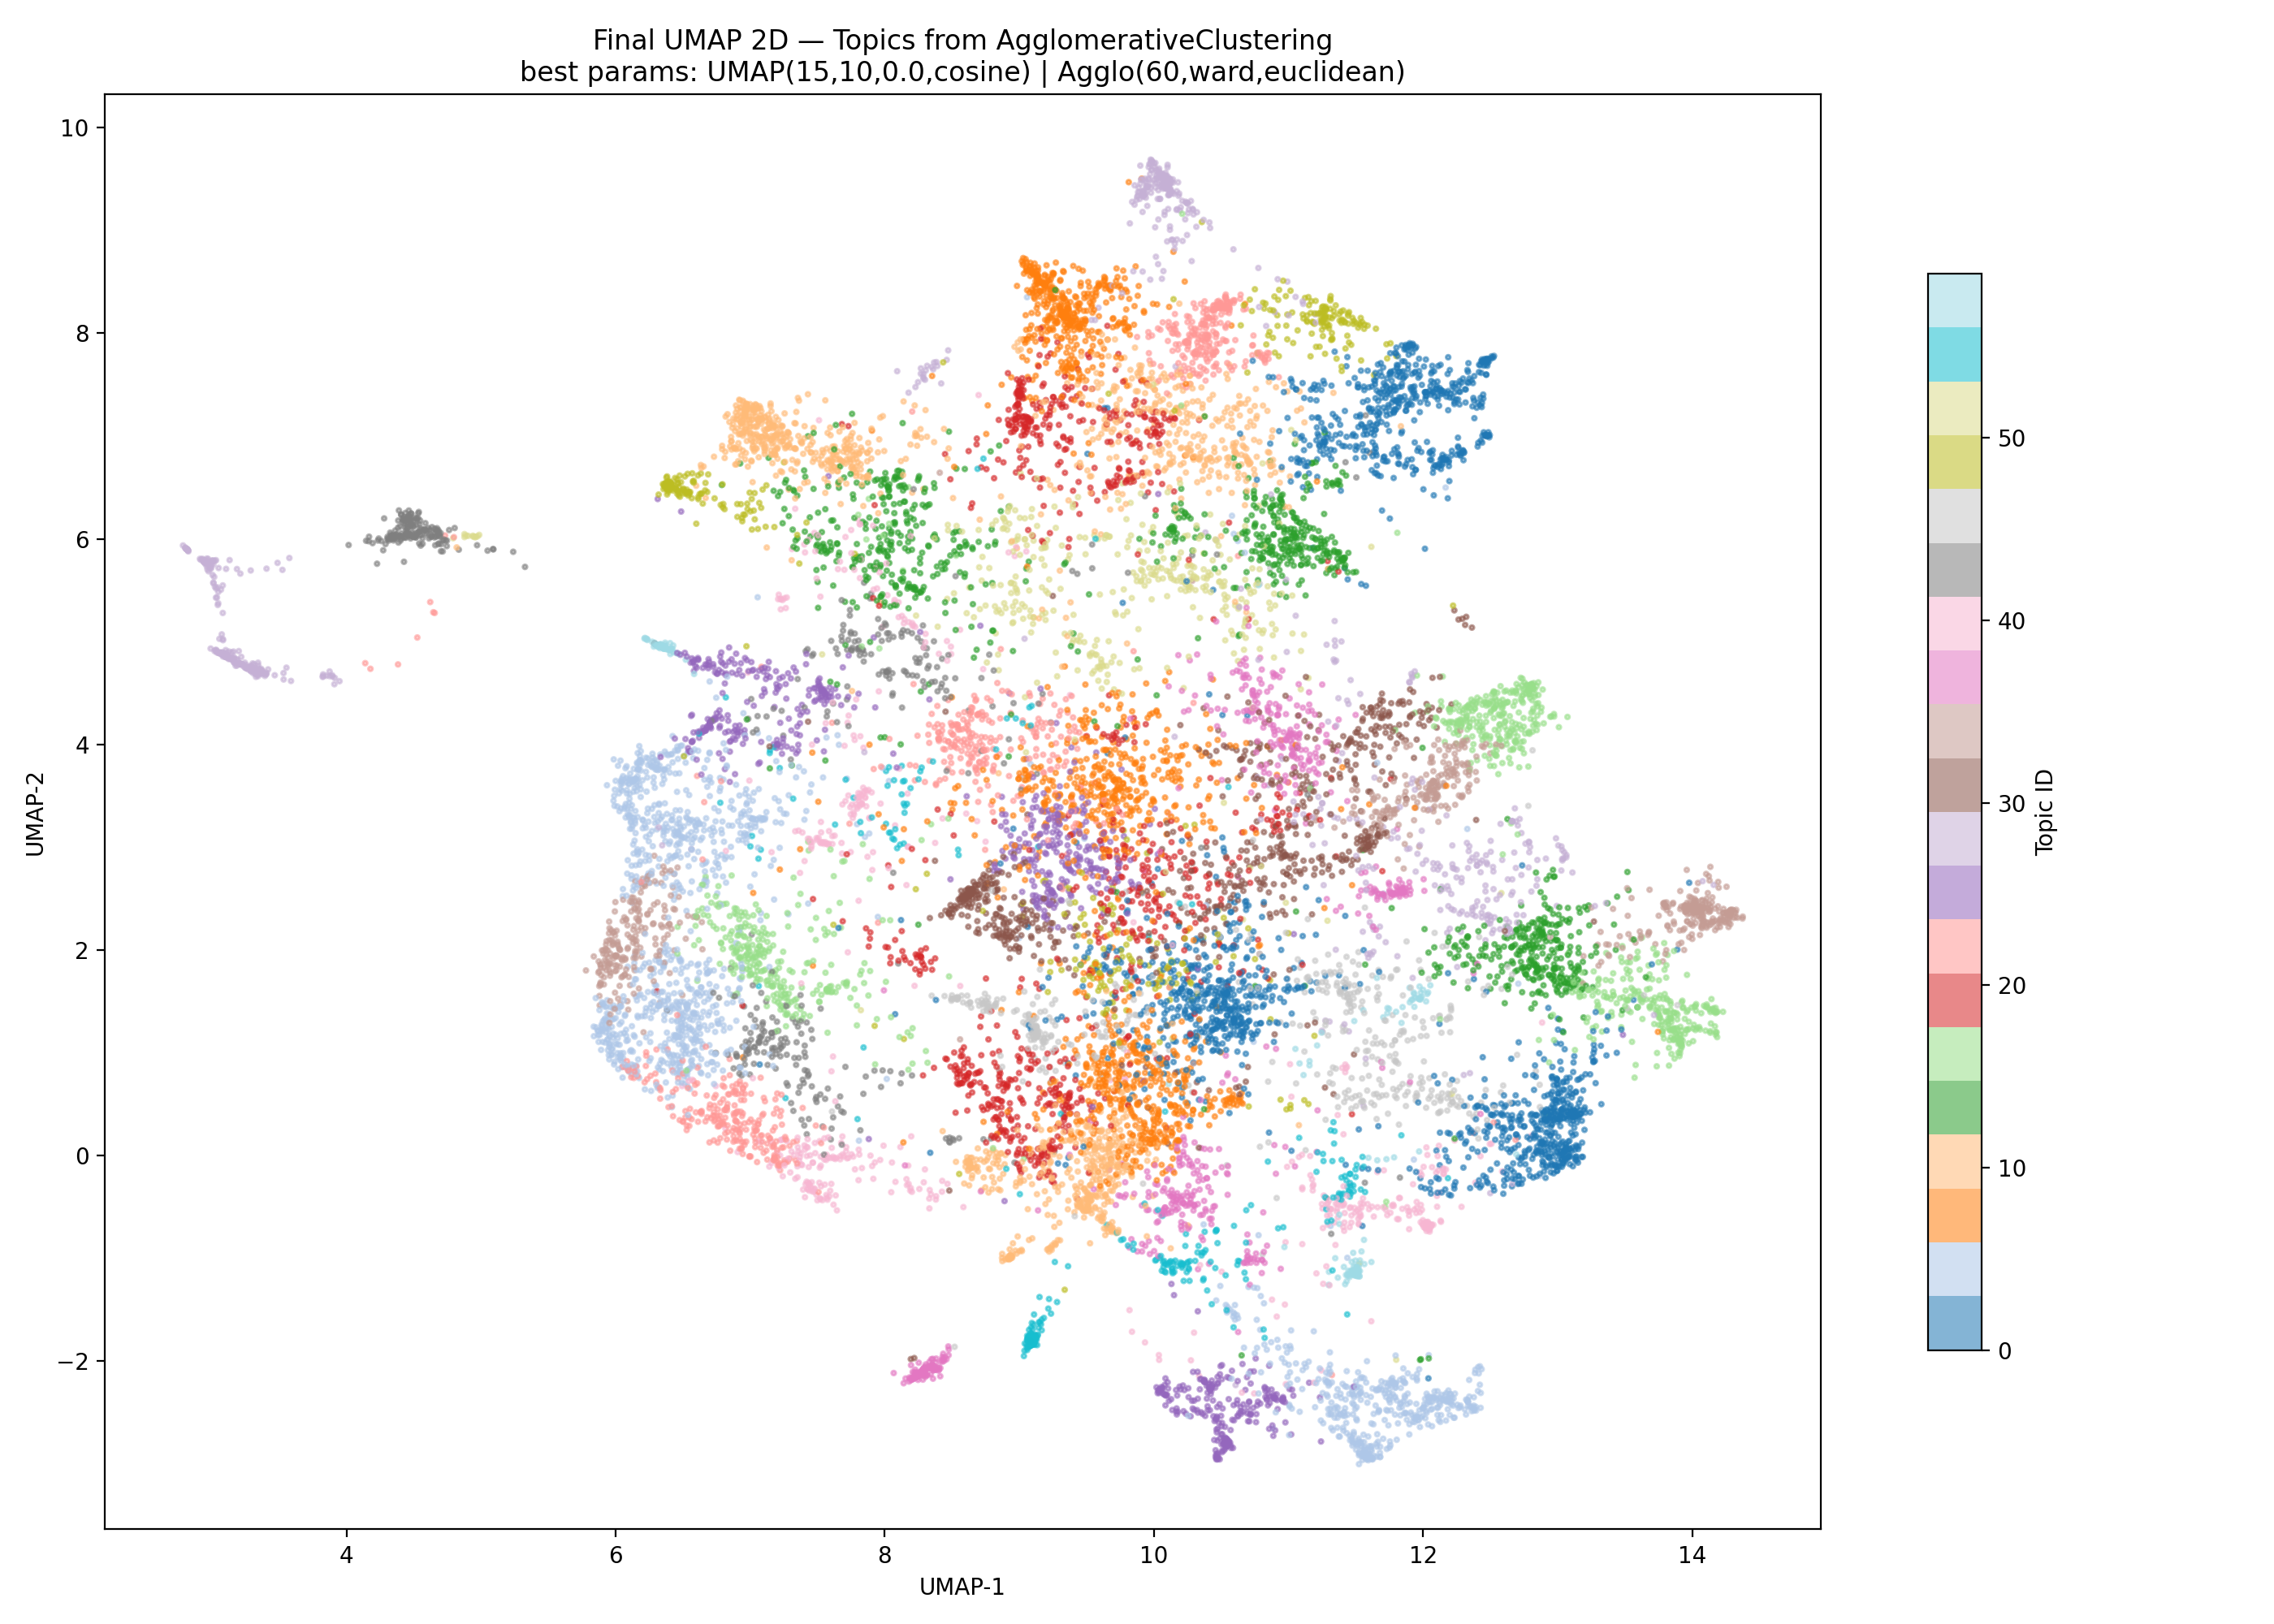
\includegraphics[width=\linewidth,height=0.52\textheight,keepaspectratio]{docx_media/image8.png}

            \capline{UMAP 投影：60 个主题在语义空间中可被稳定区分}
        \end{column}
        \begin{column}{0.48\linewidth}
            \begin{block}{聚类流程}
                \small
                文本嵌入(Specter2)\\
                \quad   $\Downarrow$\\
                UMAP 降维\\
                \quad $\Downarrow$\\
                Agglomerative 层次聚类\\
                \quad $\Downarrow$\\
                c-TF-IDF 命名与代表文献解释
            \end{block}
        \end{column}
    \end{columns}
    \begin{itemize}
        \small
        \item 识别出 \hi{60} 个主题，Silhouette \hi{0.3914}, 且\hi{无显式噪声类}。
        \item \hi{结论：} 主题团簇边界清晰，说明技术版图已经能够被稳定地表达、比较和解释
    \end{itemize}
\end{frame}

\begin{frame}{二、层次结构验证：聚类分支具有学科可解释性}
    \begin{columns}[T]
        \begin{column}{0.54\linewidth}
            \centering
            \vspace{2em}
            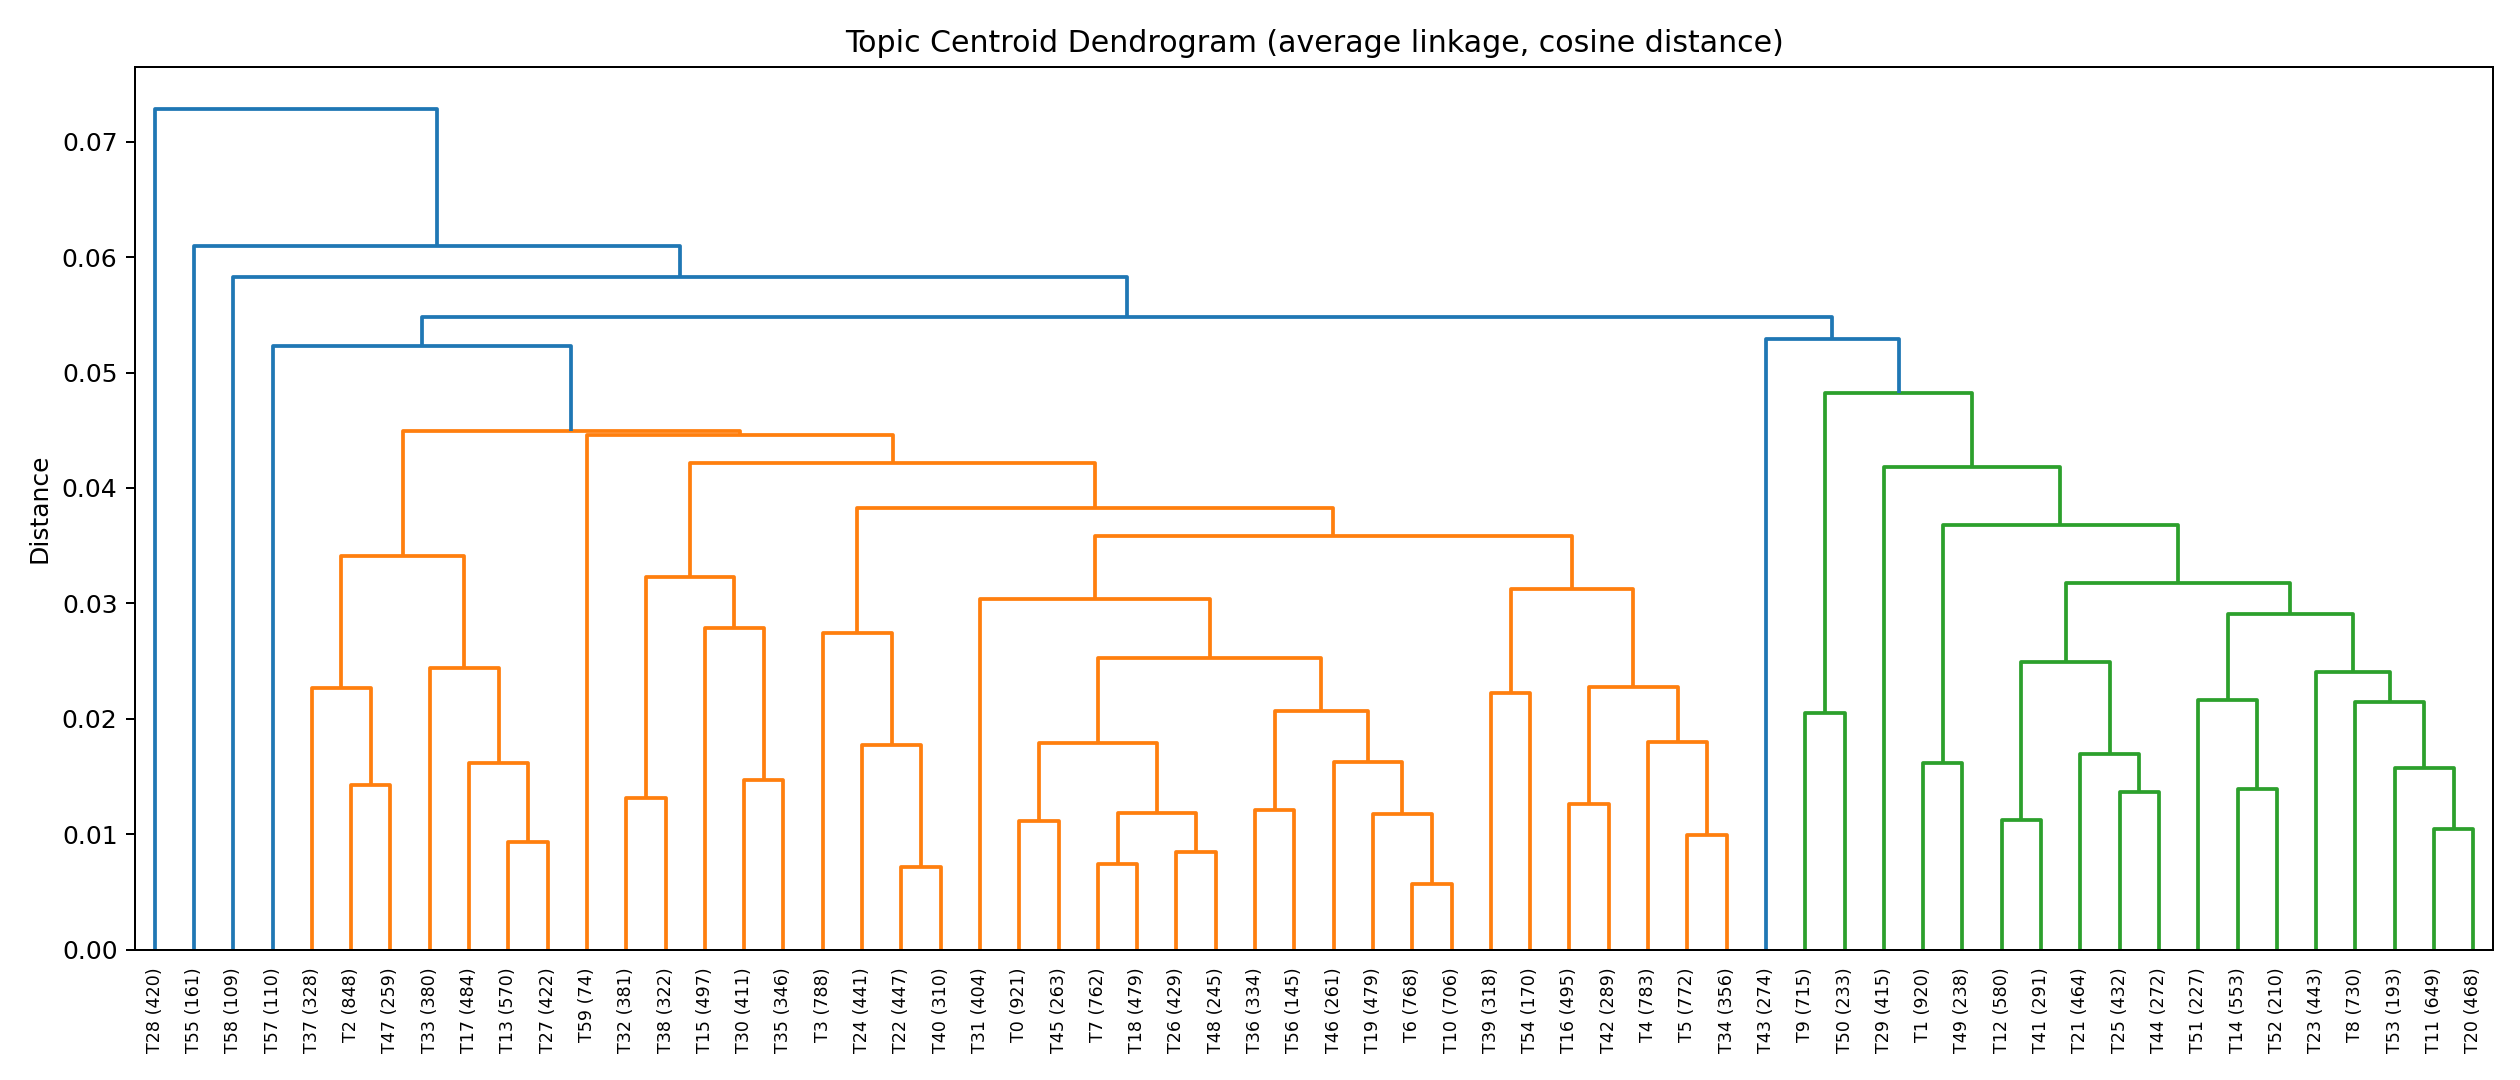
\includegraphics[width=\linewidth,height=0.52\textheight,keepaspectratio]{docx_media/image7.png}

            \capline{主题质心树状图：主题间存在稳定层次结构}
        \end{column}
        \begin{column}{0.50\linewidth}
            \small
            \begin{itemize}
                \item \textbf{AI 数据驱动：} Topic 2: \hi{故障诊断与机器学习} Topic 47: \hi{模型预测与神经网络}。
                \item \textbf{热工水利与两相流：} Topic 6: \hi{传热、流体力学} Topic 10: \hi{两相流、棒束}。
                \item \textbf{后端化学与环保：} Topic 9: \hi{水环境/海水提铀} Topic 50: \hi{气态环境/放射性碘捕获}。
            \end{itemize}
        \end{column}
    \end{columns}
    \vspace{0.5em}
    {\scriptsize \hi{结论：} 枝内主题共享底层问题与方法范式，同一层次下的枝间差异更小。
                因而该结果同时满足\hi{层次性}与\hi{文献可解释性}。}
\end{frame}

\begin{frame}{三、子领域追赶的研究分析流程}
    \begin{columns}[T]
        \begin{column}{0.48\linewidth}
            \begin{block}{步骤 1：先看趋势}
                \small
                通过分析中美两国在每个主题上的年度份额变化，识别
                \hi{catching\_up / pulling\_away / stable} 的技术追赶模式，
                并定位 cross year。
            \end{block}
            \begin{block}{步骤 2：再读代表论文}
                \small
                读取主题下的代表性论文，了解其细分领域、关注点及技术变化过程。
            \end{block}
        \end{column}
        \begin{column}{0.48\linewidth}
            \begin{block}{步骤 3：抽象追赶路径}
                \small
                把“曲线变化”与“创新类型”对应起来，
                判断它属于：
                \begin{itemize}
                    \item 应用导向型追赶
                    \item 治理管理型追赶
                    \item 基础机理型分化
                \end{itemize}
            \end{block}
            \begin{block}{解释逻辑}
                \small
                主题追赶不是总量叙事，而是
                \hi{不同子领域以不同机制、不同速度收敛或再分化}。
            \end{block}
        \end{column}
    \end{columns}
\end{frame}

\begin{frame}{应用导向主题：T2 / T9 / T10 的追赶路径}
    \scriptsize
    \begin{columns}[T]
        \begin{column}{0.32\linewidth}
            \centering
            
\includegraphics[width=\linewidth,height=0.26\textheight,keepaspectratio]{topics_papers_media/image1.png}

            \textbf{T2: AI 故障诊断}
            
            2014 年前后由负转正。代表论文以 hybrid intelligence 架构整合神经网络、数据融合与符号图，体现\hi{数据驱动运维}的快速追赶。
        \end{column}
        \begin{column}{0.32\linewidth}
            \centering
            
\includegraphics[width=\linewidth,height=0.26\textheight,keepaspectratio]{topics_papers_media/image3.png}

            \textbf{T9: 放射性化学}

            同样在 2014 年前后转正，且 2018 年后继续上升。代表论文以 PD/GO 材料实现高铀吸附容量，属于\hi{材料工艺协同型}追赶。
        \end{column}
        \begin{column}{0.32\linewidth}
            \centering
            
\includegraphics[width=\linewidth,height=0.26\textheight,keepaspectratio]{topics_papers_media/image4.png}

            \textbf{T10: 反应堆热工水力学}

            2004 年即完成超越。代表论文针对海洋环境下的传热建模，说明中国在\hi{工程场景适配型}主题上追赶更早、更快。
        \end{column}
    \end{columns}
    \vspace{0.25em}
    \begin{block}{这一组主题说明什么}
        \small
        当创新更多依赖算法集成、材料改性、工程场景建模时，中国更容易通过\hi{应用落地与工程迭代}实现份额反超。
    \end{block}
\end{frame}

\begin{frame}{治理管理主题：T13 / T27 的缓慢追赶}
    \scriptsize
    \begin{columns}[T]
        \begin{column}{0.49\linewidth}
            \centering
            
\includegraphics[width=\linewidth,height=0.30\textheight,keepaspectratio]{topics_papers_media/image5.png}

            \textbf{T13: 概率安全评价（PSA）}

            2009 年附近接近或短暂越过零点，但此后长期在零附近波动。代表论文基于大亚湾核电站总结 PSA 的开发与动态更新经验，体现的是\hi{工程实践驱动的治理能力提升}。
        \end{column}
        \begin{column}{0.49\linewidth}
            \centering
            
\includegraphics[width=\linewidth,height=0.30\textheight,keepaspectratio]{topics_papers_media/image6.png}

            \textbf{T27: 老化管理与安全管理系统}

            2011 年附近越过零点，但优势并不持续扩大。代表论文开发 SERAMIS 管理信息系统，说明这类主题的追赶依赖\hi{制度、流程和数字化工具}，收敛更慢。
        \end{column}
    \end{columns}
    \vspace{0.25em}
    \begin{block}{解释}
        \small
        治理管理类主题可以通过工程实践迅速缩小差距，但由于它们高度依赖长期规范积累与安全文化，往往\hi{难以形成持续的大幅领先}。
    \end{block}
\end{frame}

\begin{frame}{基础机理主题：T4 / T7 显示追赶并不均匀}
    \scriptsize
    \begin{columns}[T]
        \begin{column}{0.52\linewidth}
            \centering
            
\includegraphics[width=\linewidth,height=0.30\textheight,keepaspectratio]{topics_papers_media/image2.png}

            \textbf{T4: 辐照损伤与核材料}

            该主题被识别为 \hi{pulling\_away}。中国早期份额并不弱，但 2013 年后重新转负，在该领域中，
            《Molecular dynamics of single-particle impacts predicts phase diagrams for large scale pattern formation》
            这篇论文为核材料的抗辐照设计提供了全新的理论标准。说明基础理论密集型主题可能出现突破式创新，形成巨大的技术版图波动。
        \end{column}
        \begin{column}{0.44\linewidth}
            \begin{block}{T7: 核燃料与堆芯机理}
                \scriptsize
                代表论文利用 DFT 解释 U/Np/Pu 氧化物缺陷协同机制，说明燃料与堆芯主题更依赖\hi{微观机理}与长期材料知识积累。
            \end{block}
            \begin{block}{这类主题的共同特征}
                \scriptsize
                \begin{itemize}
                    \item 更依赖理论、实验平台和材料数据库
                    \item 追赶周期更长，难靠短期工程扩张完成反超
                    \item 更容易在前沿阶段重新分化
                \end{itemize}
            \end{block}
            \hi{结论：} 不是所有主题都会顺着同一条曲线追赶，基础机理赛道更容易出现重新分化。
        \end{column}
    \end{columns}
\end{frame}

\begin{frame}{四、追赶的路径与机制：赛道分化式追赶}
    \begin{columns}[T]
        \begin{column}{0.49\linewidth}
            \centering
            \includegraphics[width=\linewidth,height=0.46\textheight,keepaspectratio]{../output/cluster_results/time_evolution/figs/lead_lag_bar.png}

            \capline{主题进入年份 lead-lag 分类}
        \end{column}
        \begin{column}{0.49\linewidth}
            \centering
            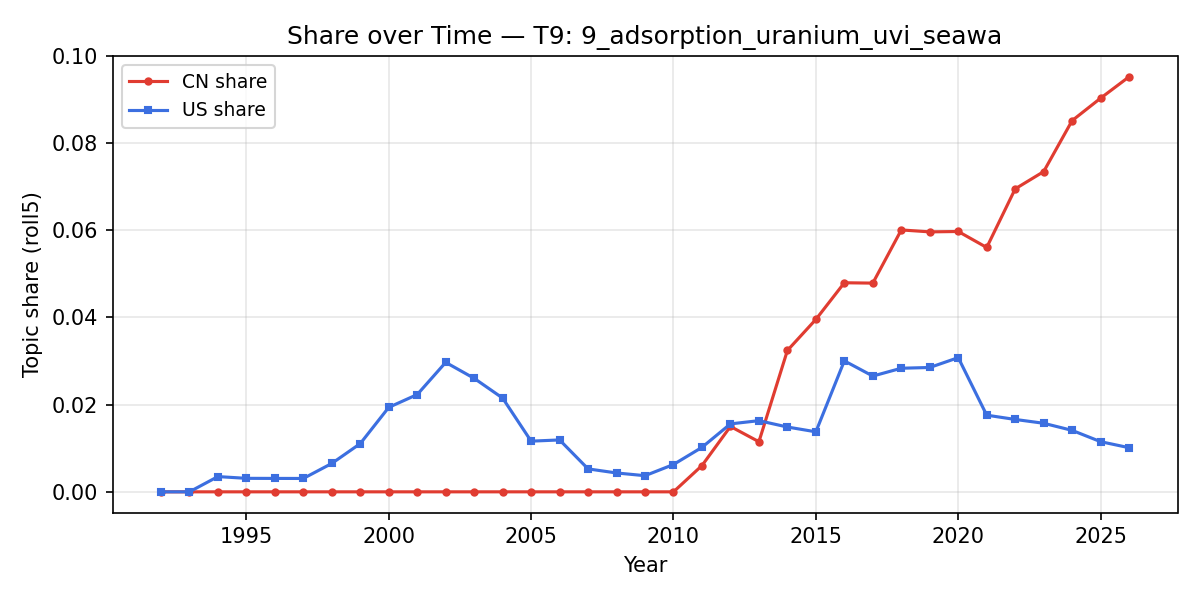
\includegraphics[width=\linewidth,height=0.46\textheight,keepaspectratio]{docx_media/image5.png}

            \capline{放射性化学类主题的追赶路径示例}
        \end{column}
    \end{columns}
    \vspace{0.2em}
    \small
    \begin{itemize}
        \item 60 个主题中，\hi{31} 个属于 catching\_up，\hi{13} 个 stable，\hi{16} 个 pulling\_away；追赶并非平均发生，而是高度依赖具体子领域。
        \item 结果发现：中国的追赶更常表现为\hi{从无到有 + 短时迸发}，是对美国已有成果的快速跟进。
        \item 从细节上看：应用导向主题追赶更快，安全治理主体尚未实现完全追赶，基础机理主题则更容易在前沿阶段重新分化。
    \end{itemize}
\end{frame}

\begin{frame}{五、总体的技术差距：从跟跑、并跑再到领跑地位转变}
    \begin{columns}[T]
        \begin{column}{0.49\linewidth}
            \centering
            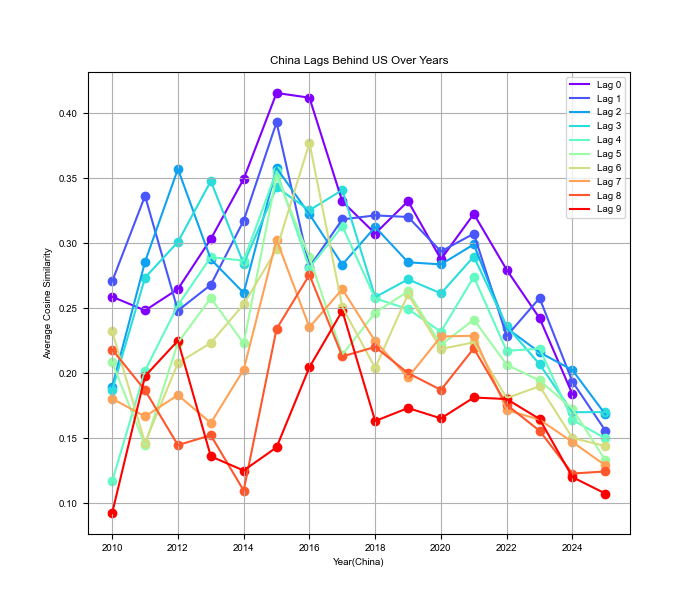
\includegraphics[width=\linewidth,height=0.46\textheight,keepaspectratio]{../cosine_similarity_China_lags_behind_US_China_year-all.png}

            \capline{中国当年主题分布与美国滞后 0--9 年分布的相似度}
        \end{column}
        \begin{column}{0.49\linewidth}
            \centering
            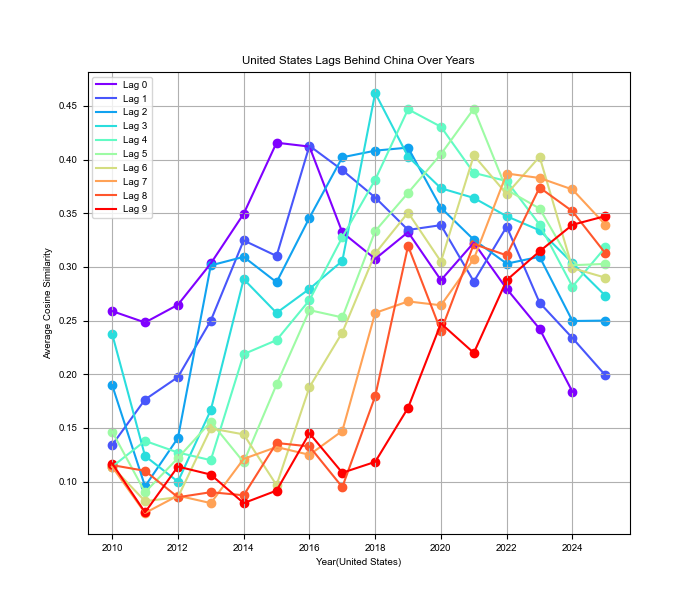
\includegraphics[width=\linewidth,height=0.46\textheight,keepaspectratio]{../cosine_similarity_US_lags_behind_China_United_States_year-all.png}

            \capline{美国当年主题分布与中国滞后 0--9 年分布的相似度}
        \end{column}
    \end{columns}
    \vspace{0.05em}
    \tiny
    \begin{block}{测度口径}
        基于 [国家, 年份] 的 topic 频次分布，比较当年结构与对方滞后结构的 multiset Jaccard 相似度。
    \end{block}
    \vspace{-0.2em}
    \begin{itemize}
        \item 中国相对美国的最优滞后多落在 \hi{0--3 年}，2014 年后多次压缩到 \hi{0--1 年}。
        \item 美国相对中国的最优滞后在 2018 年后拉长至 \hi{3--9 年}，说明中国在核领域总体上逐步超越美国的发展态势。
    \end{itemize}
\end{frame}

\begin{frame}{六、追赶的技术版图：同场竞争而非同构分布}
    \begin{columns}[T]
        \begin{column}{0.64\linewidth}
            \centering
            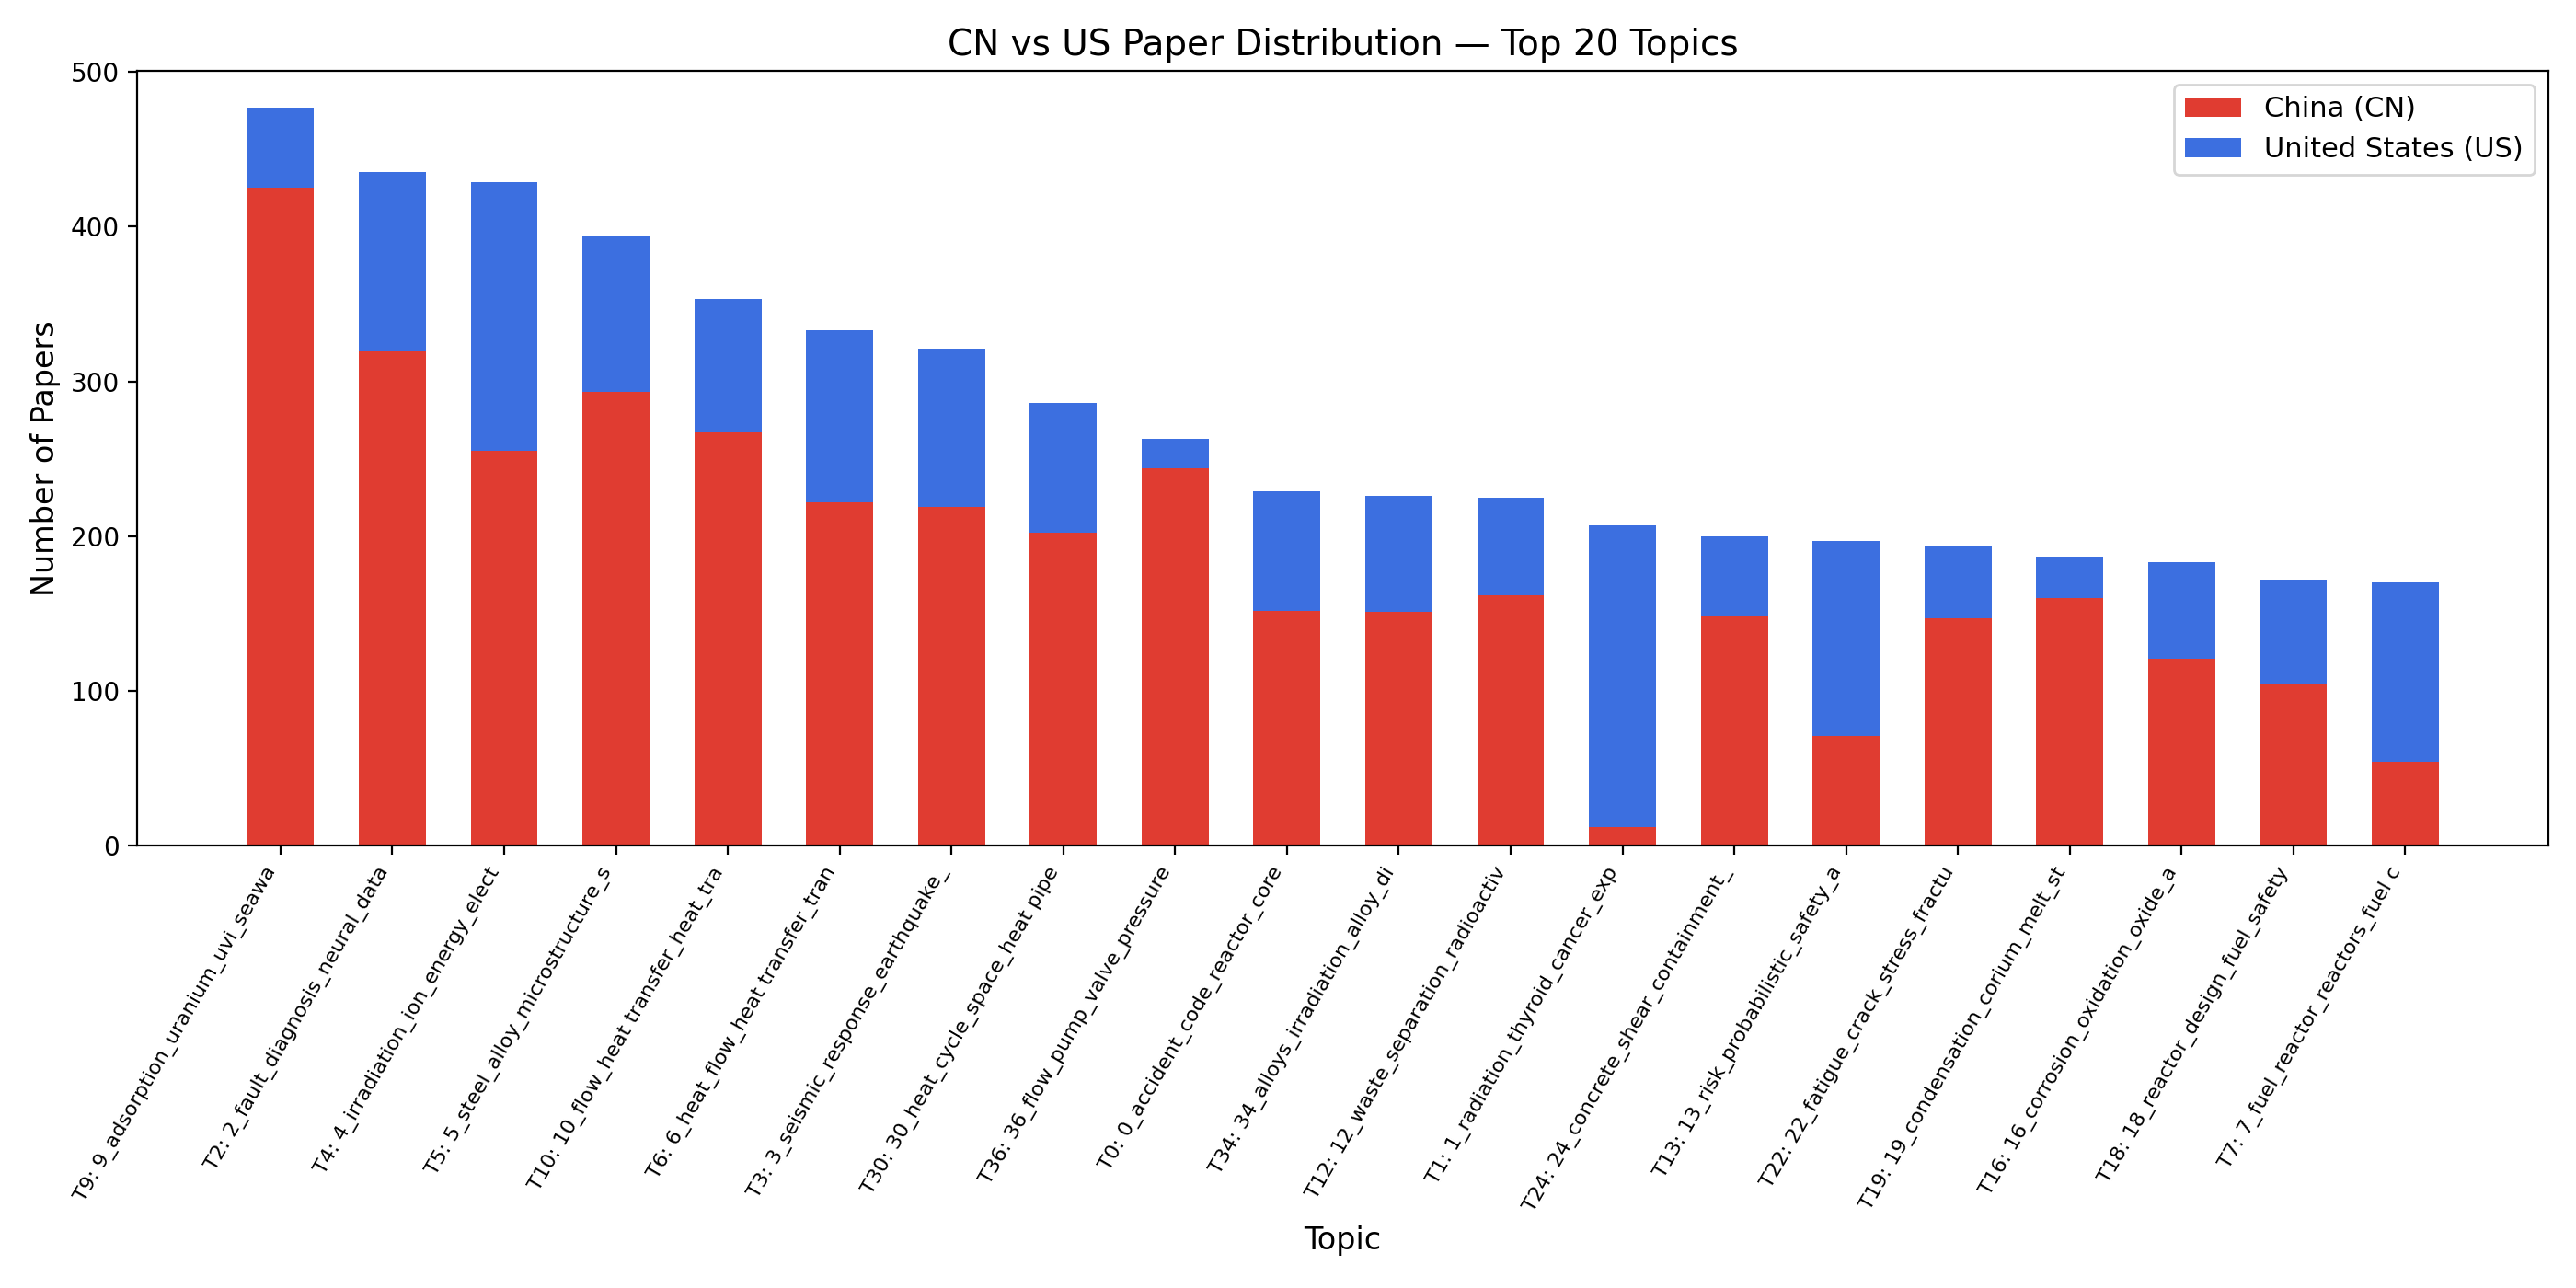
\includegraphics[width=\linewidth,height=0.62\textheight,keepaspectratio]{docx_media/image9.png}
        \end{column}
        \begin{column}{0.32\linewidth}
            \begin{block}{关键数字}
                \small
                主题总数：\hi{60}\\
                CN 覆盖：\hi{58/60}\\
                US 覆盖：\hi{60/60}\\
                JS distance：\hi{0.3022}
            \end{block}
            \begin{block}{判断}
                \small
                已经是“同场竞争”，\\
                但不是“同构分布”。
            \end{block}
        \end{column}
    \end{columns}
\end{frame}

\begin{frame}{七、前沿能力：结构差距与方向分化}
    \begin{columns}[T]
        \begin{column}{0.49\linewidth}
            \centering
            \includegraphics[width=\linewidth,height=0.46\textheight,keepaspectratio]{../output/cluster_results/capability_gap/frontier_topic_distribution.png}

            \capline{US frontier 与 CN frontier 的主题分布差异}
        \end{column}
        \begin{column}{0.49\linewidth}
            \centering
            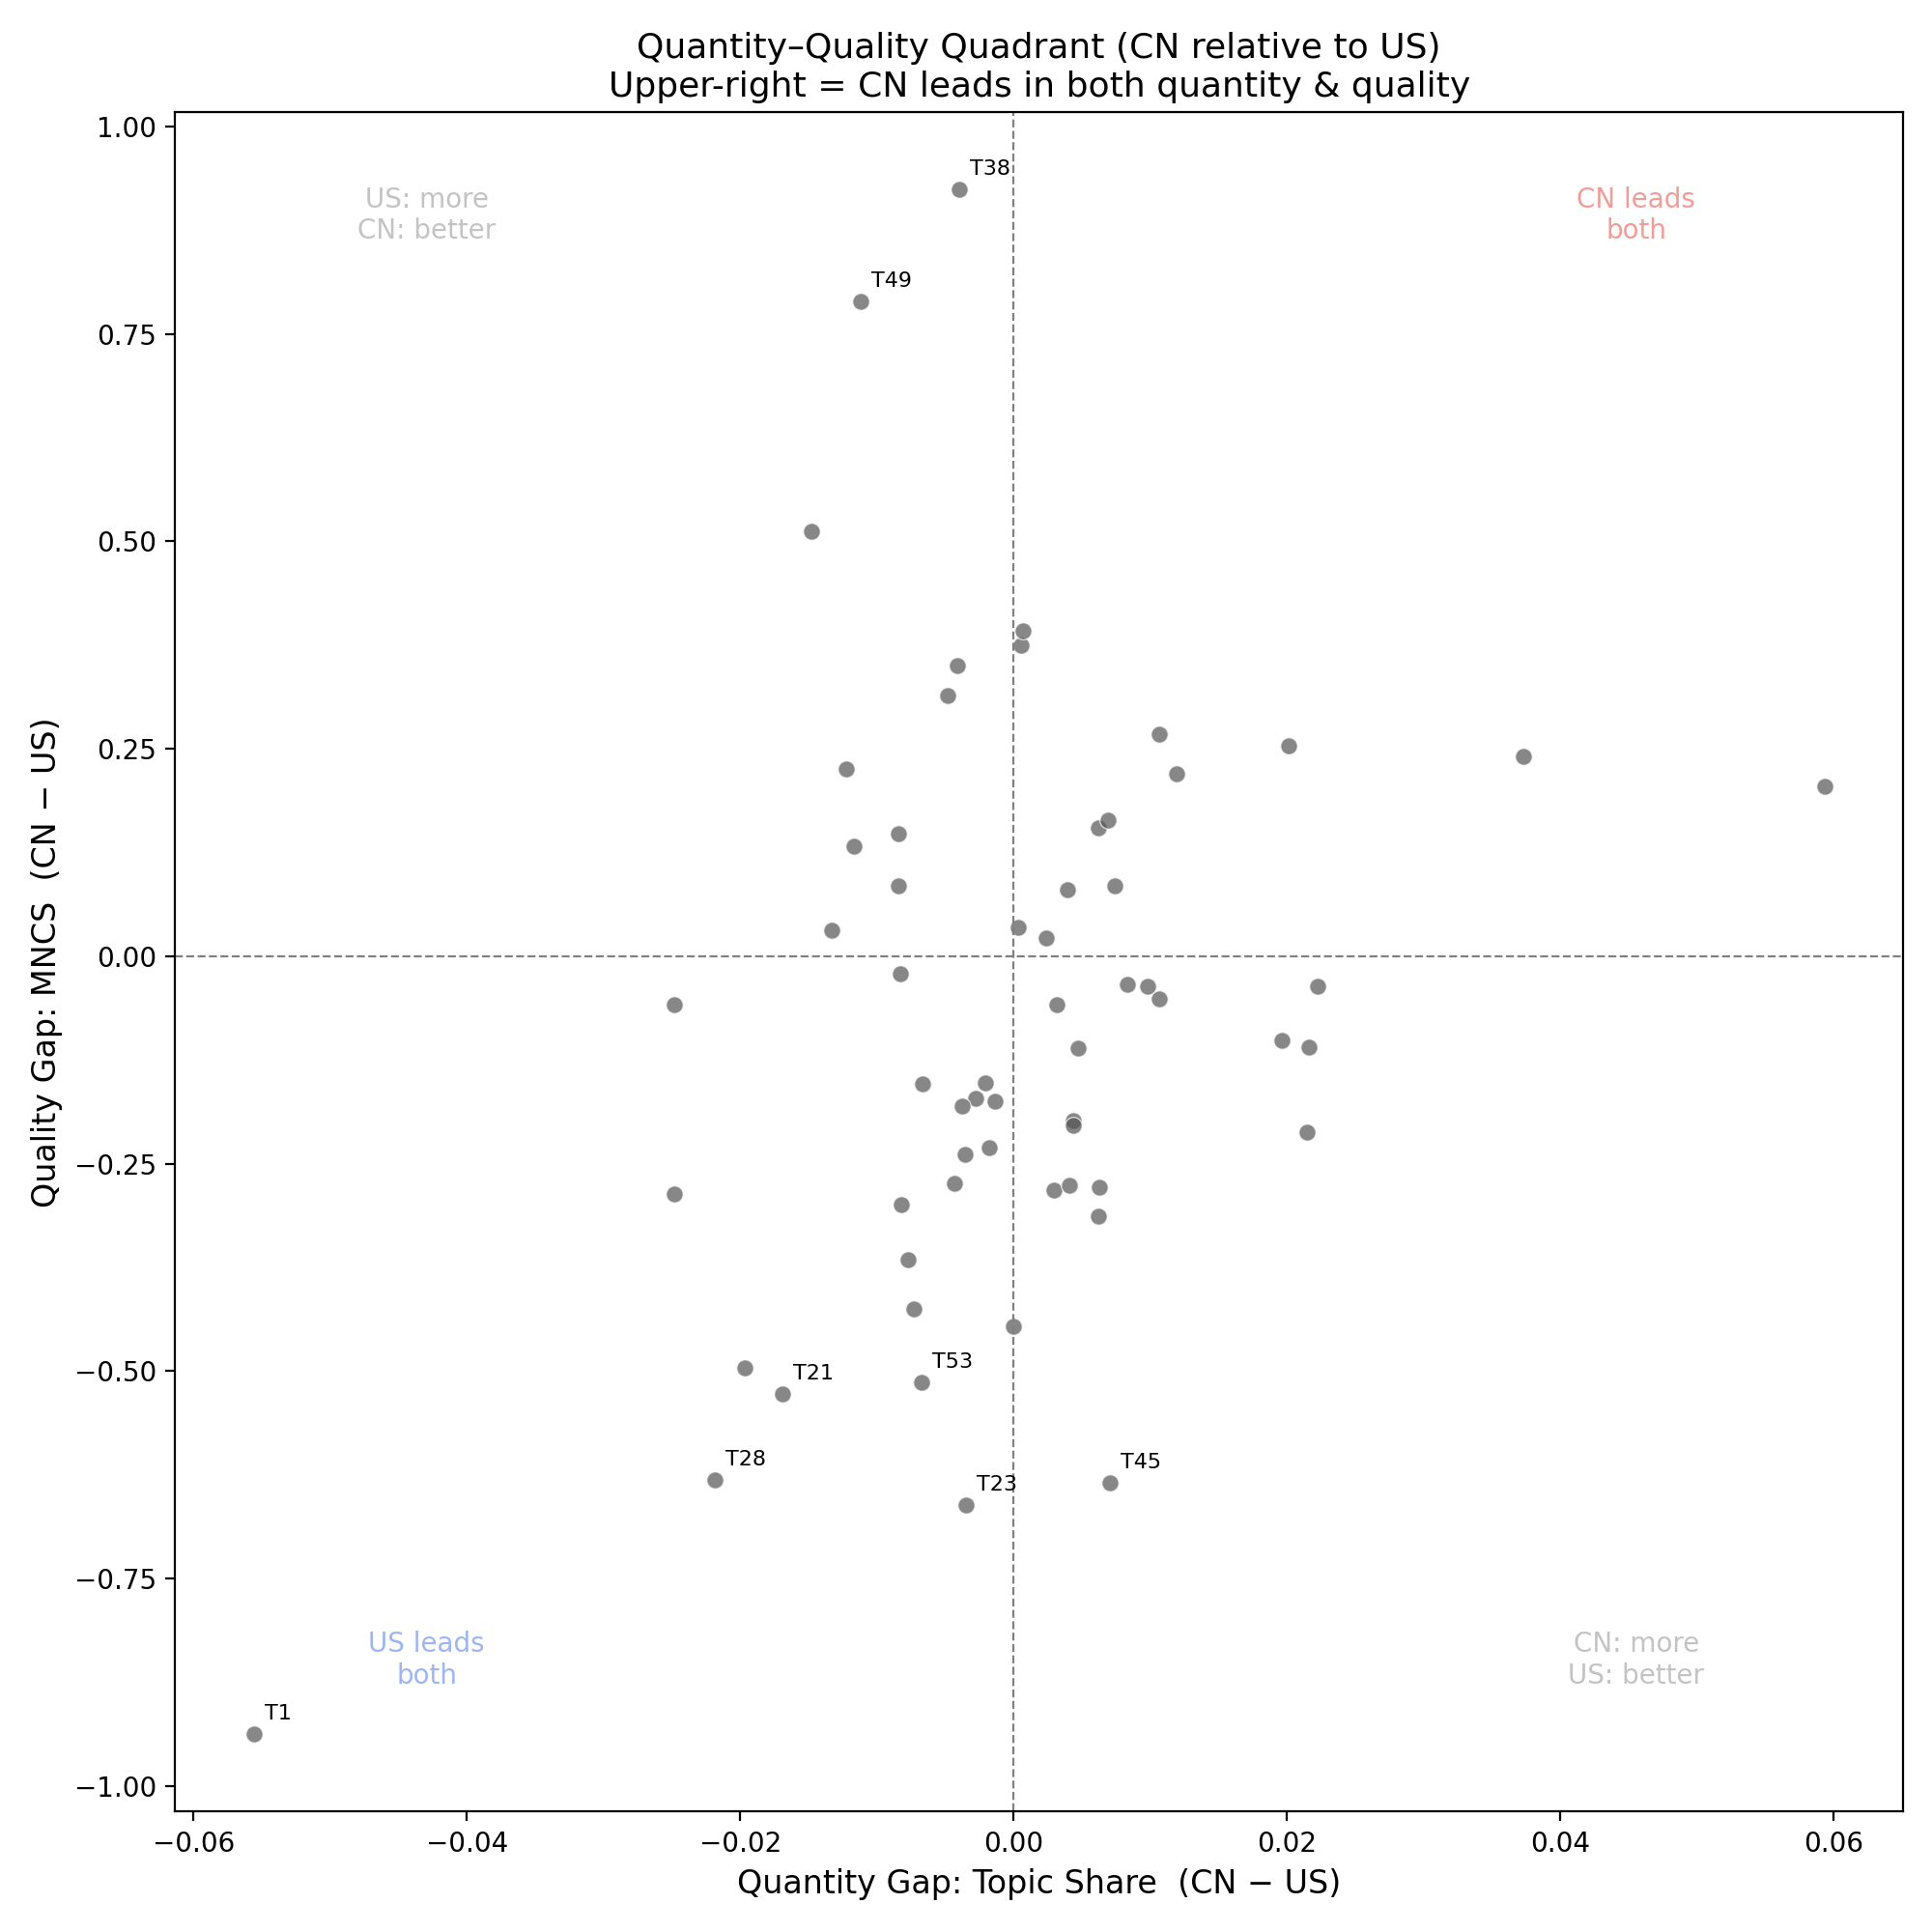
\includegraphics[width=\linewidth,height=0.46\textheight,keepaspectratio]{docx_media/image6.png}

            \capline{数量-质量象限：高产出不必然对应高质量}
        \end{column}
    \end{columns}
    \vspace{0.2em}
    \scriptsize
    \begin{itemize}
        \item 总体主题结构差距（JS distance）为 \hi{0.3022}，但 2021--2025 前沿窗口下的 frontier JS distance 已上升到 \hi{0.4734}，两国的研究重心出现了分化。
        \item 中美两国都分别在不同领域培育出了核心优势（美国：辐射暴露、radiocesium/forest、安全不确定性等；中国：核能利用、核废料处理等）。
        \item \hi{阶段性判断：} 前沿能力的差距正在显现，且呈现出核心优势方向分化的特点。
    \end{itemize}
\end{frame}

\section{结论与下一阶段目标}

\begin{frame}{阶段性结论}
    \begin{itemize}
        \item 中国已进入绝大多数主题赛道，且在大部分赛道上实现了快速追赶。
        \item 在应用导向型、治理管理型、基础机理型主题上，追赶路径呈现出差异化特征。
        \item 总体上看，中国实现了对美国核领域的技术超越，且技术优势愈加明显。
        \item 前沿领域，国家间的结构差距正在显现，主题方向呈现分化趋势。
    \end{itemize}
\end{frame}

\begin{frame}{下一阶段：从图论比较中美在版图中的相对位置}
    \begin{columns}[T]
        \begin{column}{0.49\linewidth}
            \centering
            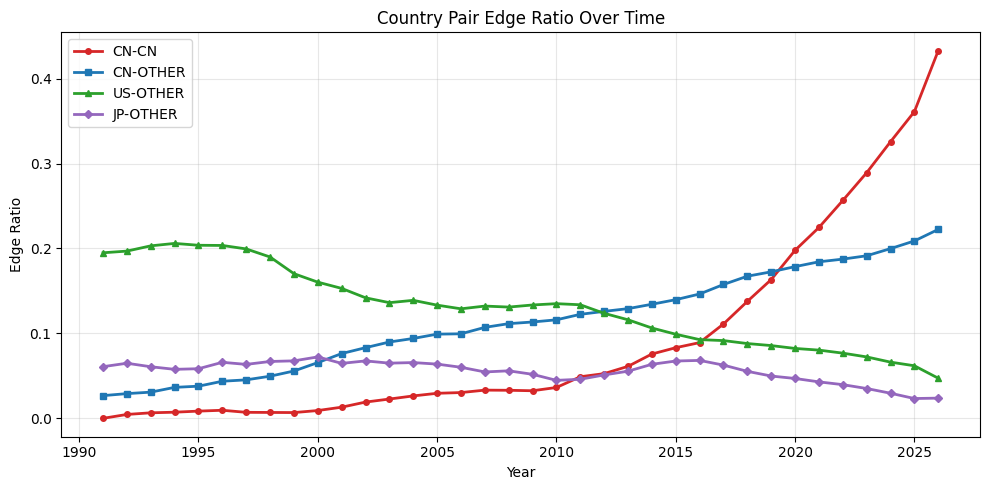
\includegraphics[width=\linewidth,height=0.44\textheight,keepaspectratio]{docx_media/image1.png}

            \capline{跨国边比例随时间变化}
        \end{column}
        \begin{column}{0.49\linewidth}
            \centering
            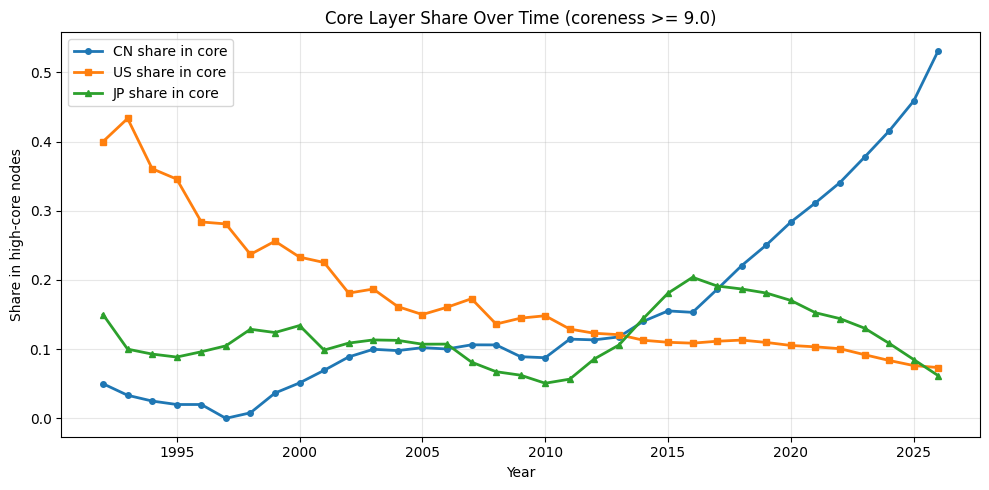
\includegraphics[width=\linewidth,height=0.44\textheight,keepaspectratio]{docx_media/image2.png}

            \capline{高核层占比随时间变化}
        \end{column}
    \end{columns}
    \vspace{0.2em}
    \small
    \begin{itemize}
        \item 下一阶段将正式构建\hi{动态语义网络}，比较中美论文在核心层、边缘层和跨国连接中的相对位置变化。
        \item 重点检验三个问题：跨国连接是否增强、中国论文是否由外围进入核心、主题边界与国家边界何者更强。
        \item 这一步将把“进入同一版图”进一步推进到“在版图中的\hi{位置追赶}”。
    \end{itemize}
\end{frame}

\begin{frame}{下一阶段：用图论对照潜在知识邻近与实际知识调用}
    \begin{columns}[T]
        \begin{column}{0.62\linewidth}
            \centering
            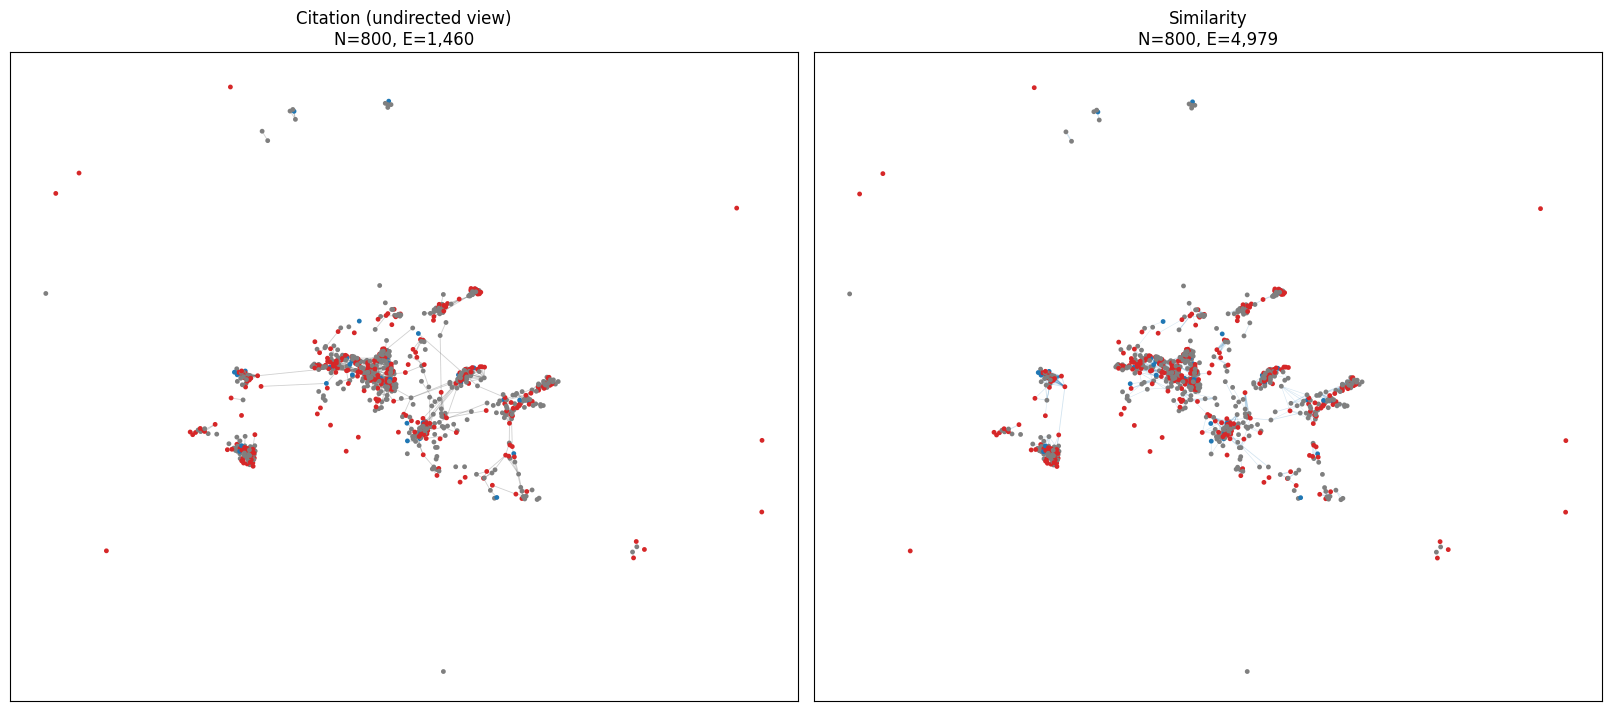
\includegraphics[width=\linewidth,height=0.50\textheight,keepaspectratio]{docx_media/image3.png}

            \capline{引文网络图与相似度网络图的结构对照}
        \end{column}
        \begin{column}{0.34\linewidth}
            \centering
            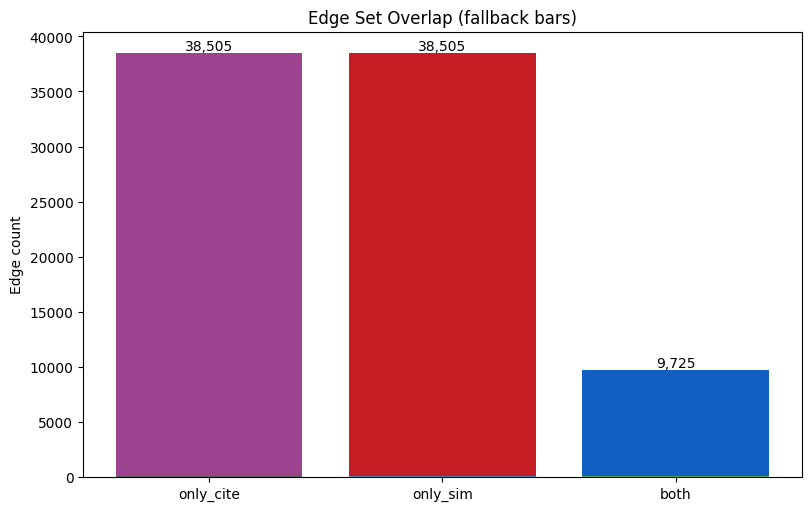
\includegraphics[width=\linewidth,height=0.24\textheight,keepaspectratio]{docx_media/image4.png}

            \vspace{0.3em}
            \begin{block}{初步图示}
                \scriptsize
                both：\hi{9,725}\\
                Jaccard：\hi{0.2526}
            \end{block}
        \end{column}
    \end{columns}
    \vspace{0.1em}
    \small
    \begin{itemize}
        \item 下一阶段将以\hi{相似网络}刻画潜在知识邻近，以\hi{引文网络}刻画实际知识调用，比较两类网络的重叠、偏离与方向性差异。
        \item 核心问题是：中美技术追赶究竟表现为“结构靠近”，还是已经转化为“真实知识吸收与扩散”。
    \end{itemize}
\end{frame}

\begin{frame}{下一阶段工作}
    \begin{itemize}
        \item 将\hi{“主题结构差距 - 发展路线差异 - 前沿能力差距 - 知识扩散方式”}整理为统一论文主线。
        \item 以图论方式正式比较语义网络与引文网络，构建\hi{引文预测模型}，识别中美技术追赶的结构机制与知识流动机制。
        \item 选取少数代表性主题做\hi{案例深化}，把 topic trend、代表论文与网络位置变化连成完整分析链条。
        \item 整理所有研究内容，形成一篇高质量的研究论文。
    \end{itemize}
\end{frame}

\begin{frame}
    \begin{center}
        {\Huge\calligra Thanks!}
    \end{center}
\end{frame}

\end{document}
